


\begin{frame}[plain,c]
\begin{center}
{\Huge \bf Optional reading for Lecture \thislecture}
\end{center}
\end{frame}

%
%
%

\begin{frame}{Estimating $\int_{a}^{b} \frac{dz}{({\rho}^2+z^2)^{3/2}}$}

We can prove that:
\begin{equation*}
  \int_{a}^{b} \frac{dz}{({\rho}^2+z^2)^{3/2}} = \frac{z}{{\rho}^{2}(z^{2}+{\rho}^{2})^{1/2}} \biggr\rvert_{a}^{b}
\end{equation*}

\vspace{0.2cm}

{\small
One way to calculate this integral is to change variables ($z \rightarrow u$) and perform an integration over the variable u.
A clever variable transformation will leave us with a much simpler integral to calculate.\\

Let's try the following variable transformation:
\begin{equation*}
  z \rightarrow u = tan^{-1}\Big(\frac{z}{{\rho}})\Big)
\end{equation*}

Therefore:
\begin{equation*}
   z = {\rho} tan(u) \;\;\;\; and \;\;\;\;
  dz = {\rho} \Big( tan(u) \Big) du \Rightarrow dz = \frac{{\rho}}{cos^{2}(u)} du
\end{equation*}
}
\end{frame}

%
%
%

\begin{frame}{Estimating $\int_{a}^{b} \frac{dz}{({\rho}^2+z^2)^{3/2}}$}

{\small
With that variable transformation, the integrand becomes:
\begin{equation*}
   \frac{1}{({\rho}^2+z^2)^{3/2}} \rightarrow
     \frac{1}{({\rho}^{2}tan^{2}(u)+{\rho}^{2})^{3/2}} =
     \frac{1}{{\rho}^{3}(tan^{2}(u)+1)^{3/2}} =
     \frac{1}{{\rho}^{3}( \frac{sin^{2}(u)}{cos^{2}(u)}+1)^{3/2}} =
\end{equation*}
\begin{equation*}
   = \frac{1}{{\rho}^{3}( \frac{sin^{2}(u)+cos^{2}(u)}{cos^{2}(u)})^{3/2}} =
     \frac{1}{{\rho}^{3}( \frac{1}{cos^{2}(u)})^{3/2}} =
     \frac{cos^{3}(u)}{{\rho}^{3}}
\end{equation*}

Therefore:
\begin{equation*}
  \int_{a}^{b} \frac{dz}{({\rho}^2+z^2)^{3/2}} =
    \int_{u(a)}^{u(b)} \Big( \frac{cos^{3}(u)}{{\rho}^{3}} \Big) \Big( \frac{{\rho}}{cos^{2}(u)} du \Big) =
    \frac{1}{{\rho}^2} \int_{u(a)}^{u(b)} cos(u) du =
\end{equation*}
\begin{equation*}
   = \frac{1}{{\rho}^2} sin(u) \biggr\rvert_{u(a)}^{u(b)}
   = \frac{1}{{\rho}^2} sin\Big[ tan^{-1}\Big((\frac{z}{{\rho}})\Big) \Big]  \biggr\rvert_{a}^{b}
\end{equation*}
}
\end{frame}

%
%
%

\begin{frame}{Estimating $\int_{a}^{b} \frac{dz}{({\rho}^2+z^2)^{3/2}}$}

\begin{columns}
  \begin{column}{0.30\textwidth}
    {\small
     In order to evaluate the term
     \begin{equation*}
       sin\Big[ tan^{-1}\Big(\frac{z}{\rho}\Big) \Big] \biggr\rvert_{a}^{b}
     \end{equation*}
     appearing in the previous expression,
     consider the triangle below.\\
    }
    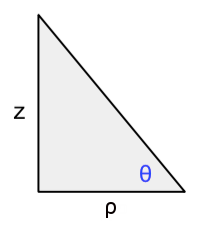
\includegraphics[width=0.85\textwidth]{./images/schematics/triangle_for_integral_in_wire_magnetic_field_calc.png}
  \end{column}
  \begin{column}{0.70\textwidth}
  {\small
    We have:
    \begin{equation*}
      tan(\theta) = \frac{z}{{\rho}} \Rightarrow
      \theta = tan^{-1}\Big( \frac{z}{{\rho}} \Big)  \Rightarrow
      sin(\theta) = sin\Big[ tan^{-1}\Big( \frac{z}{{\rho}} \Big) \Big]
    \end{equation*}
    But:
    \begin{equation*}
      sin(\theta) = \frac{z}{(z^2+{\rho}^2)^{1/2}}
    \end{equation*}
    Therefore:
    \begin{equation*}
       sin\Big[ tan^{-1}\Big( \frac{z}{{\rho}} \Big) \Big] = \frac{z}{(z^2+{\rho}^2)^{1/2}}
    \end{equation*}
    So, indeed, we showed that:
    \begin{equation*}
      \int_{a}^{b} \frac{dz}{({\rho}^2+z^2)^{3/2}} = \frac{z}{{\rho}^{2}(z^{2}+{{\rho}^{2}})^{1/2}} \biggr\rvert_{a}^{b}
    \end{equation*}
  }
  \end{column}
\end{columns}

\end{frame}

% ------------------------------------------------------------------------------
% ------------------------------------------------------------------------------

%
% Worked example :
%

{
\problemslide

%
%
%

\begin{frame}{Worked example: Magnetic field of circular loop}

  \begin{blockexmplque}{Question}
    Calculate the magnetic field along the axis of a circular loop
    carrying a steady current $I$.
    \vspace{0.1cm}
    \begin{center}
      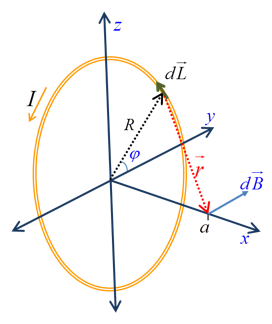
\includegraphics[width=0.35\textwidth]{./images/problems/lect05_circular_loop_b_field.png}\\
    \end{center}
  \end{blockexmplque}

\end{frame}

%
%
%

\begin{frame}{Worked example: Magnetic field of circular loop}

  To calculate the magnetic field $\vec{B}$ produced
  by the circular loop, we will use the Biot-Savart law:
  \begin{equation*}
     \vec{B} = \int_{L} d\vec{B} =
      \frac{\mu_0 I}{4\pi} \int_{L} \frac{d\vec{\ell} \times \vec{r}}{r^3}
  \end{equation*}

  The loop axis is the $x$-axis.
  For a point at distance $a$ on that axis,
  the location vector $\vec{r}_{axis}$
  can be written as:
  \begin{equation*}
     \vec{r}_{axis} = \Big(a, 0, 0\Big)
  \end{equation*}

  The circular loop is on the $y-z$ plane ($x$ = 0).
  The location vector $\vec{r}_{loop}$
  for any point on the loop is:
  \begin{equation*}
     \vec{r}_{loop} = \Big(0, R cos\phi, R sin\phi \Big)
  \end{equation*}

  The vector $\vec{r}$ connecting points on the loop
  and the loop axis is:
  \begin{equation*}
      \vec{r} = \vec{r}_{axis} - \vec{r}_{loop} =
      \Big(a, 0, 0\Big) - \Big(0, R cos\phi, R sin\phi \Big) =
      \Big(a, -R cos\phi, -R sin\phi \Big)
  \end{equation*}

\end{frame}

%
%
%

\begin{frame}{Worked example: Magnetic field of circular loop}

  Therefore, the magnitude of $\vec{r}$ is:
  \begin{equation*}
      r = |\vec{r}| = \Big(a^2 + R^2 cos^{2}\phi + R^2 sin^{2}\phi \Big)^{1/2} =  \Big(a^2 + R^2 \Big)^{1/2}
  \end{equation*}

  The element $d\vec{\ell}$ that is
  tangential to the loop can be written as:
  \begin{equation*}
          d\vec{\ell} = \Big(0, - R sin\phi, R cos\phi \Big) d\phi
  \end{equation*}

  The cross-product of $d\vec{\ell}$ and  $\vec{r}$ is:
  \begin{equation*}
      d\vec{\ell} \times \vec{r} =
      \Big(0, - R sin\phi, R cos\phi \Big) \times
      \Big(a, -R cos\phi, -R sin\phi \Big)  d\phi \Rightarrow
  \end{equation*}

  \begin{equation*}
      d\vec{\ell} \times \vec{r} =
      \Big(R^2, a R cos\phi, a R sin\phi \Big) d\phi
  \end{equation*}

\end{frame}

%
%
%

\begin{frame}{Worked example: Magnetic field of circular loop}

  Substituting everything into the Biot-Savart equation, we have:
  \begin{equation*}
     \vec{B} = \frac{\mu_0 I}{4\pi}
        \int_{L} \frac{d\vec{\ell} \times \vec{r}}{r^3}
             = \frac{\mu_0 I}{4\pi}
        \int_{0}^{2\pi}
        \frac{\Big(R^2, a R cos\phi, a R sin\phi \Big)}{\Big(a^2 + R^2 \Big)^{3/2}} d\phi
        \Rightarrow
  \end{equation*}

  \begin{equation*}
     \vec{B} = \frac{\mu_0 I}{4\pi \Big(a^2 + R^2 \Big)^{3/2}}
       \int_{0}^{2\pi} \Big(R^2, a R cos\phi, a R sin\phi \Big) d\phi
        \Rightarrow
  \end{equation*}

  \begin{equation*}
     \vec{B} = \frac{\mu_0 I}{4\pi \Big(a^2 + R^2 \Big)^{3/2}}
        \Big(R^2 \int_{0}^{2\pi} d\phi ,
             a R \int_{0}^{2\pi}  cos\phi d\phi ,
             a R \int_{0}^{2\pi}  sin\phi d\phi \Big)
        \Rightarrow
  \end{equation*}

  % \begin{equation*}
  %    \vec{B} = \frac{\mu_0 I}{4\pi \Big(a^2 + R^2 \Big)^{3/2}}
  %                   \Big(R^2 2\pi, 0 , 0 \Big)
  %       \Rightarrow
  % \end{equation*}

  \begin{equation*}
     \vec{B} = \frac{\mu_0 I R^2}{2 \Big(a^2 + R^2 \Big)^{3/2}}
                    \Big(1, 0 , 0 \Big)
  \end{equation*}

\end{frame}

} % Worked example


% ------------------------------------------------------------------------------
% ------------------------------------------------------------------------------

%
% Worked example :
%

{
\problemslide

%
%
%

\begin{frame}{Worked example: Field of straight wire semi-circular bent}

  \begin{blockexmplque}{Question}
    An infinitely long wire carries a current $I$.
    It is bent so as to have a semi-circular detour around the origin,
    with radius $R$. Calculate the magnetic field $\vec{B}$ at the origin.
  \end{blockexmplque}

  \begin{center}
    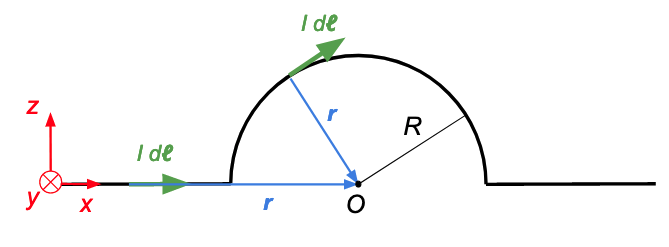
\includegraphics[width=0.70\textwidth]{./images/problems/lect05_wire_with_semicircular_bent_2}\\
  \end{center}

  The field $\vec{B}$ of a current element $Id\vec{\ell}$
  is given by the Biot-Savart law:
  \begin{equation*}
    d\vec{B} = \frac{\mu_0I}{4\pi} \frac{d\vec{\ell} \times \vec{r}}{r^3}
  \end{equation*}

\end{frame}

%
%
%

\begin{frame}{Worked example: Field of straight wire semi-circular bent}

The straight parts of the wire do not contribute to the magnetic field at the
origin $O$ since, as it can be seen from the schematic above, for these parts
of the wire, $d\vec{\ell}$ and $\vec{r}$ are parallel and, therefore:
\begin{equation*}
  d\vec{\ell} \times \vec{r} = 0
\end{equation*}

Only the semicircular bent contributes to the magnetic field at the origin.
On that bent, $d\vec{\ell}$ and $\vec{r}$ are always perpendicular
to each other and the law of Biot-Savart can be simplified as:
\begin{equation*}
  d\vec{B} = \frac{\mu_0I}{4\pi} \frac{r d\ell}{r^3} \hat{y}
           = \frac{\mu_0I}{4\pi} \frac{d\ell}{r^2} \hat{y} \xRightarrow{r=R, d\ell=Rd\theta}
  d\vec{B} = \frac{\mu_0I}{4\pi R} d\theta \hat{y}
\end{equation*}

Thefore, the magnetic field due to the full semi-circular bent is given by:
\begin{equation*}
  \vec{B} = \int_{semicircle} d\vec{B} =
     \frac{\mu_0I}{4\pi R} \Bigg( \int_{0}^{\pi} d\theta \Bigg) \hat{y} \Rightarrow
  \vec{B} = \frac{\mu_0I}{4 R} \hat{y}
\end{equation*}


\end{frame}


} % Worked example


% ------------------------------------------------------------------------------
% ------------------------------------------------------------------------------

%
% Worked example :
%

{
\problemslide

%
%
%

\begin{frame}{Worked example: Field of rotating cylindrical shell}

  \begin{blockexmplque}{Question}
    Consider a cylindrical shell of radius $R$ and length $L$,
    carrying charge with surface charge density $\sigma$ and rotating with
    angular velocity $\omega$.\\
    Find the mangnetic field $\vec{B}$ at point $P$,
    at distance $d$ from the end of the shell, on the cylinder axis.
  \end{blockexmplque}

  The most general form of the Biot-Savart law, giving the magnetic
  field $\vec{B}(\vec{r})$ due to an arbitrary volume current density $\vec{j}$ is:
  \begin{equation*}
    \vec{B}(\vec{r}) = \frac{\mu_0}{4\pi}
      \int_{\tau} d\tau^\prime
      \frac{\vec{j}(\pvec{r}') \times (\vec{r}-\pvec{r}')}{|(\vec{r}-\pvec{r}')|^3}
  \end{equation*}
  where the integration is over volume $\tau$.

  For a surface current density $\vec{K}$, on surface $S$ the above simplifies to:
  \begin{equation*}
    \vec{B}(\vec{r}) = \frac{\mu_0}{4\pi}
      \int_{S} dS^\prime
      \frac{\vec{K}(\pvec{r}') \times (\vec{r}-\pvec{r}')}{|(\vec{r}-\pvec{r}')|^3}
  \end{equation*}

\end{frame}

%
%
%

\begin{frame}{Worked example: Field of rotating cylindrical shell}

The previous expression, using the coordinate system, and the definitions
of vectors $\vec{r}$ and $\pvec{r}'$ shown in the figure below,
yields the following expression for the magnetic field $\vec{B}$ at point $P$.
\begin{equation*}
  \vec{B} = \frac{\mu_0}{4\pi}
    \int_{cylinder} dS^\prime
    \frac{\vec{K}(\pvec{r}') \times \hat{r}}{r^2}
\end{equation*}

\begin{center}
  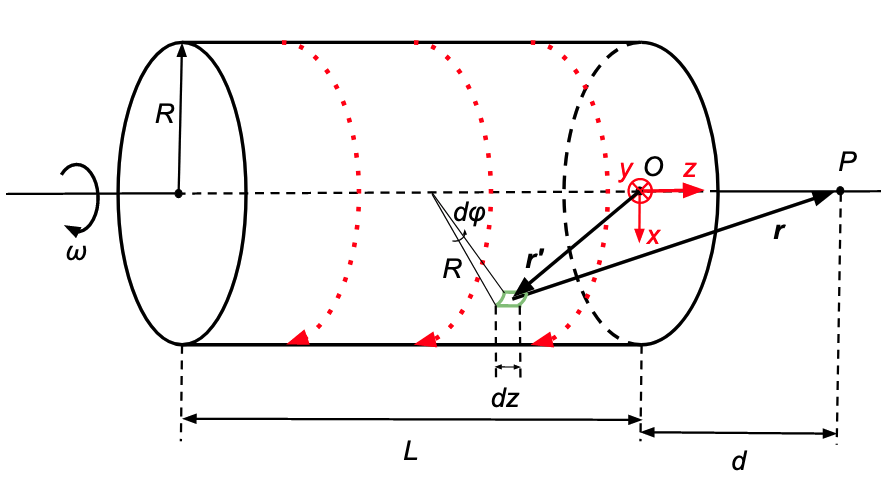
\includegraphics[width=0.80\textwidth]{./images/problems/lect05_bfield_of_rotating_cylindrical_shell_a_1}\\
 \end{center}

\end{frame}

%
%
%

\begin{frame}{Worked example: Field of rotating cylindrical shell}

It is useful to draw a projection of the previous schematic on the $xz$ plane.
Angles and distances which are going to be used later, are defined here.
\begin{center}
  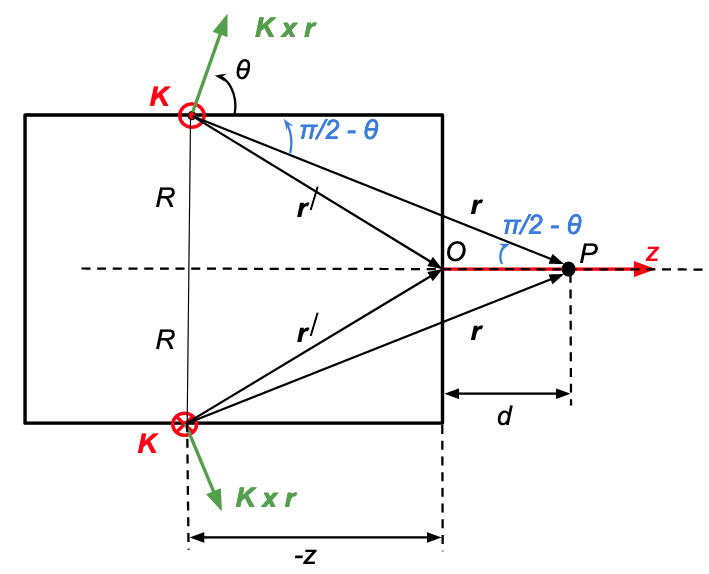
\includegraphics[width=0.70\textwidth]{./images/problems/lect05_bfield_of_rotating_cylindrical_shell_b_1}\\
\end{center}

\end{frame}

%
%
%

\begin{frame}{Worked example: Field of rotating cylindrical shell}

If $\vec{u}$ is the velocity of each point on the surface of the cylinder,
the surface current density $\vec{K}$ is given by:
\begin{equation*}
  \vec{K} = \sigma \vec{u} = \sigma \omega R \hat{\phi}
\end{equation*}
where  $\hat{\phi}$ is the azimuthal unit vector.

Since $\vec{K}(\pvec{r}')$ and $\hat{r}$ are perpendicular,
the magnitude of $\vec{K}(\pvec{r}') \times \hat{r}$ is:
\begin{equation*}
  |\vec{K}(\pvec{r}') \times \hat{r}| =
    |\vec{K}(\pvec{r}')| \cancelto{1}{|\hat{r}|} \cancelto{1}{sin\frac{\pi}{2}} =
    |\vec{K}(\pvec{r}')| = \sigma \omega R
\end{equation*}

Due to symmetry, only the $z$ component of
$\vec{K}(\pvec{r}') \times \hat{r}$ will contribute to the magnetic field,
as the other components cancel out. The $z$ component is:

\begin{equation*}
  \vec{K}(\pvec{r}') \times \hat{r} \rvert_{z} =
    \sigma \omega R cos\theta
\end{equation*}

\end{frame}

%
%
%

\begin{frame}{Worked example: Field of rotating cylindrical shell}

From the schematic shown a projection of the cylinder on the $xz$ plane,
we can see that:
\begin{equation*}
  cos\theta = sin(\frac{\pi}{2}-\theta) = \frac{R}{r}
\end{equation*}

Therefore, the only non-vanishing contribution of $\vec{K}(\pvec{r}') \times \hat{r}$
to the magnetic field at $P$ can be written as:
\begin{equation*}
  \vec{K}(\pvec{r}') \times \hat{r}  =
    \frac{\sigma \omega R^2}{r} \hat{z}
\end{equation*}

Substituting the above into Biot-Savart's expression for the magnetic field
at $P$, and using $dS^\prime = R d\phi dz$, we find:
\begin{equation*}
  \vec{B} =
    % \frac{\mu_0}{4\pi}
    % \int_{cylinder} R d\phi dz
    % \frac{\frac{\sigma \omega R^2}{r} \hat{z}}{r^2} =
    \hat{z} \frac{\mu_0 \sigma \omega R^3}{4\pi}
    \int_{cylinder} d\phi dz \frac{1}{r^3}  =
    \hat{z} \frac{\mu_0 \sigma \omega R^3}{2}
    \int_{-L}^{0} \frac{dz}{r^3}
\end{equation*}

\end{frame}

%
%
%

\begin{frame}{Worked example: Field of rotating cylindrical shell}

To carry out the integration, we need to express $r$ in terms of $z$.
Looking the previous schematic, we see that:
\begin{equation*}
  r^2 = R^2 + (d+z)^2
\end{equation*}

Therefore, the magnetic field $\vec{B}$ at $P$ is given by:
\begin{equation*}
  \vec{B} =
    \hat{z} \frac{\mu_0 \sigma \omega R^3}{2}
    \int_{-L}^{0} \frac{dz}{\Big( R^2 + (d+z)^2 \Big)^{3/2}} \xRightarrow{\ell = d+z}
\end{equation*}
\begin{equation*}
  \vec{B} =
  \hat{z} \frac{\mu_0 \sigma \omega R^3}{2}
  \int_{d-L}^{d} \frac{d\ell}{\Big( R^2 + \ell^2 \Big)^{3/2}}
\end{equation*}

Earlier in this lecture (field of infinite straight conductor), we proved that:
\begin{equation*}
  \int_{a}^{b} \frac{dz}{({\rho}^2+z^2)^{3/2}} = \frac{z}{{\rho}^{2}(z^{2}+{\rho}^{2})^{1/2}} \biggr\rvert_{a}^{b}
\end{equation*}

\end{frame}

%
%
%

\begin{frame}{Worked example: Field of rotating cylindrical shell}

Using the above expression to help us evaluate the integral,
we find for the magnetic field $\vec{B}$ at $P$:

\begin{equation*}
  \vec{B} =
  \hat{z} \frac{\mu_0 \sigma \omega R^3}{2}
  \frac{\ell}{R^{2}({\ell}^{2}+R^{2})^{1/2}} \biggr\rvert_{d-L}^{L} \Rightarrow
\end{equation*}

\begin{equation*}
  \vec{B} =
  \hat{z} \frac{\mu_0 \sigma \omega R^3}{2}
  \Big\{
  \frac{L}{R^{2}(L^{2}+R^{2})^{1/2}} -
  \frac{(d-L)}{R^{2}((d-L)^{2}+R^{2})^{1/2}}
  \Big\} \Rightarrow
\end{equation*}

\begin{equation*}
  \vec{B} =
  \hat{z} \frac{\mu_0 \sigma \omega R}{2}
  \Big\{
  \frac{L}{\sqrt{L^{2}+R^{2}}} -
  \frac{(d-L)}{\sqrt{(d-L)^{2}+R^{2}}}
  \Big\}
\end{equation*}

\end{frame}

%
%
%

\begin{frame}{Worked example: Field of rotating hemisphere}

  \begin{columns}
    \begin{column}{0.60\textwidth}
      \centering
      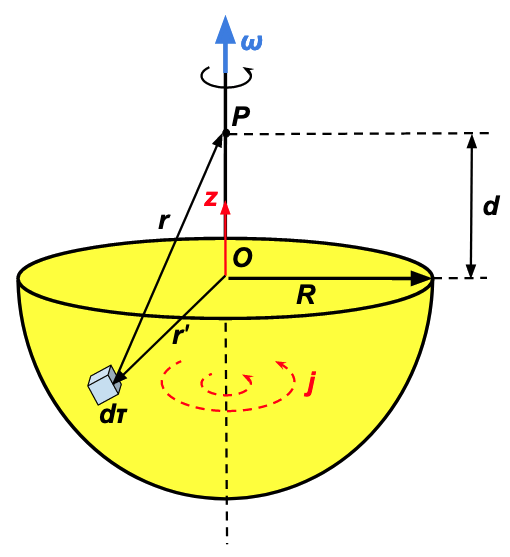
\includegraphics[width=0.95\textwidth]{./images/problems/lect05_bfield_of_rotating_semisphere_a_1}\\
    \end{column}
    \begin{column}{0.38\textwidth}
      If you have calculated the magnetic field of a rotating
      cyclindrical shell, you can also try to calculate the field of
      hemisphere of radius $R$ and volume charge density $\rho$,
      rotating with angular velocity $\omega$,
      at distance $d$ above its centre.
    \end{column}
  \end{columns}

\end{frame}

} % Worked example


% ------------------------------------------------------------------------------
% ------------------------------------------------------------------------------

%
% Worked example :
%

{
\problemslide

%
%
%

\begin{frame}{Worked example: Field of current element}

  \begin{blockexmplque}{Question}
    A current element $Id\vec{\ell}$ is located at the origin.
    The current is in the direction of the $+z$ axis.
    Is the $x$ component of the the field at a point $P$$(x,y,z)$:
    \begin{itemize}
      \item 0,
      \item $\displaystyle \frac{\mu_0 I}{4\pi} \frac{y}{(x^2+y^2+z^2)^{3/2}} d\ell$, or
      \item $\displaystyle \frac{\mu_0 I}{4\pi} \frac{x}{(x^2+y^2+z^2)^{3/2}} d\ell$?
    \end{itemize}
    Justify your answer.
  \end{blockexmplque}

  The magnetic field $\vec{B}$ of the current element $Id\vec{\ell}$
  is given by the Biot-Savart law:
  \begin{equation*}
    d\vec{B} = \frac{\mu_0 I}{4\pi} \frac{d\vec{\ell} \times \vec{r}}{r^3}
  \end{equation*}

\end{frame}

%
%
%

\begin{frame}{Worked example: Field of current element}

  \begin{columns}
    \begin{column}{0.44\textwidth}
       \begin{center}
         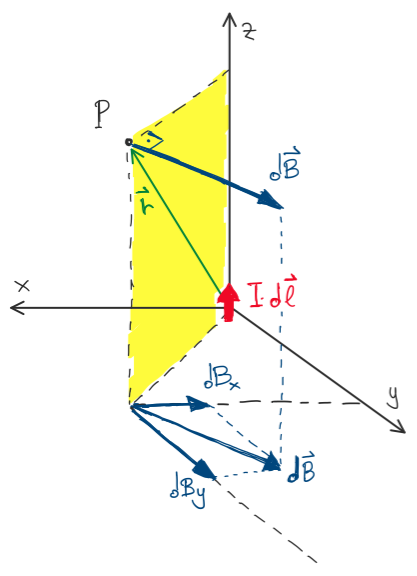
\includegraphics[width=0.99\textwidth]{./images/problems/lect05_current_element_at_origin}\\
        \end{center}
    \end{column}
    \begin{column}{0.55\textwidth}
      \begin{equation*}
        d\vec{B} = \frac{\mu_0I}{4\pi} \frac{d\vec{\ell} \times \vec{r}}{r^3}
      \end{equation*}
      \\\vspace{0.4cm}
      where, for the given problem (see schematic on the left):\\
      \begin{equation*}
        d\vec{\ell} = \Big(0,0,d\ell\Big)
      \end{equation*}
      \begin{equation*}
        \vec{r} = \Big(x,y,z\Big)
      \end{equation*}
      \begin{equation*}
        r = |\vec{r}| = \Big(x^2 + y^2 + z^2\Big)^{1/2}
      \end{equation*}
    \end{column}
  \end{columns}

\end{frame}

%
%
%

\begin{frame}{Worked example: Field of current element}

The cross-product $d\vec{\ell} \times \vec{r}$ can be written as:
\begin{equation*}
  d\vec{\ell} \times \vec{r} =
   \left|
    \begin{array}{ccc}
      \hat{x} & \hat{y} & \hat{z}    \\
            0 &       0 &      d\ell \\
            x &       y &       z    \\
    \end{array}
   \right|
   =
   \left|
    \begin{array}{cc}
            0 &  d\ell \\
            y &   z    \\
    \end{array}
   \right|
   \hat{x} -
   \left|
    \begin{array}{cc}
            0 &  d\ell \\
            x &   z    \\
    \end{array}
   \right|
   \hat{y} +
   \left|
    \begin{array}{cc}
            0 &  0 \\
            x &  y \\
    \end{array}
   \right|
   \hat{z}
\end{equation*}

\begin{equation*}
 = \Big( -y d\ell \Big) \hat{x} - \Big( -x d\ell \Big) \hat{y} + 0 \hat{y}
 = \Big( -y, x, 0 \Big) d\ell
\end{equation*}

Therefore, the magnetic field at $P$, due to the element $Id\vec{\ell}$, is:
\begin{equation*}
  d\vec{B} = \frac{\mu_0I}{4\pi}
    \frac{\Big( -y, x, 0 \Big) d\ell}{\Big(x^2 + y^2 + z^2\Big)^{3/2}}
\end{equation*}

which has an $x$-component given by:
\begin{equation*}
  dB_x = - \frac{\mu_0I}{4\pi}
    \frac{y d\ell}{\Big(x^2 + y^2 + z^2\Big)^{3/2}}
\end{equation*}

\end{frame}

} % Worked example


% ------------------------------------------------------------------------------
% ------------------------------------------------------------------------------

%
% Worked example :
%

{
\problemslide

\begin{frame}{Worked example: Bainbridge's mass spectrometer}

  \begin{blockexmplque}{Question}
    Bainbridge’s mass spectrometer, shown in the figure below,
    separates ions having the same velocity.
    \vspace{0.3cm}
    \begin{columns}
      \begin{column}{0.01\textwidth}
      \end{column}
      \begin{column}{0.59\textwidth}
      Positive ions, after entering through slits S$_1$ and S$_2$,
      pass through a velocity selector composed of an electric field $\vec{E}$
      pointing to the right, produced by the charged plates P and P$^\prime$,
      and a magnetic field $\vec{B}$, pointing out of the page,
      perpendicular to $\vec{E}$ and the ion path. The ions that then pass
      without deviation through the crossed $\vec{E}$ and $\vec{B}$ fields
      enter a region of a second magnetic field $\vec{B}^\prime$, also pointing
      out of the page, where they are made to follow circular paths.
      \end{column}
      \begin{column}{0.40\textwidth}
        \begin{center}
          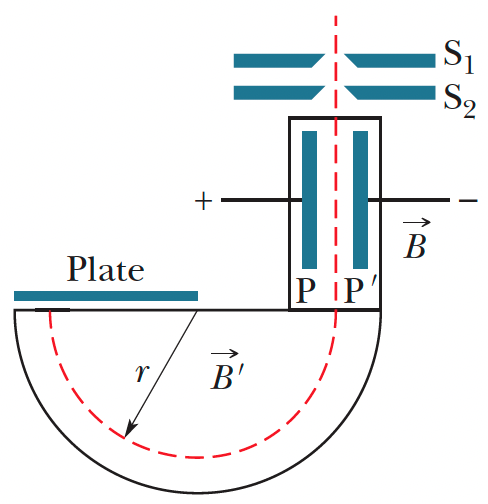
\includegraphics[width=0.99\textwidth]{./images/problems/lect05_bainbridge_1}\\
        \end{center}
      \end{column}
    \end{columns}
  \end{blockexmplque}

\end{frame}

%
%
%

\begin{frame}{Worked example: Bainbridge's mass spectrometer}

  \begin{blockexmplque}{Question}
    A photographic plate (or a modern detector) registers their arrival.
    Show that, for the ions,
    \begin{equation*}
      \frac{q}{m} = \frac{E}{rBB'}
    \end{equation*}
    where $q$ ($m$) is the charge (mass) of the ion,
    and $r$ is the radius of the circular orbit.
  \end{blockexmplque}

  After entering through slits $S_1$ and $S_2$, the ions experience
  electric and magnetic forces.
  The magnitudes of these forces are

  \begin{equation*}
    {F}_{E} = q |\vec{E}| = q E
  \end{equation*}

  \begin{equation*}
    {F}_{B} = q|\vec{u} \times \vec{B}| = q u B
  \end{equation*}

\end{frame}

%
%
%

\begin{frame}{Worked example: Bainbridge's mass spectrometer}

  Since ions pass the area of the crossed $\vec{E}$ and $\vec{B}$ fields
  without deviation, the electric and magnetic forces must be canceling
  each other out.
  \begin{equation*}
    {F}_{E} = {F}_{B}
  \end{equation*}

  The above, yields the following expression for $u$:
  \begin{equation*}
    q E = q u B \Rightarrow u = \frac{E}{B}
  \end{equation*}

  In the region where $\pvec{B}'$ exists, the ion follows a circular path
  with the magnetic force providing centripetal acceleration:
  \begin{equation*}
    m \frac{u^2}{r} = q |\vec{u} \times \pvec{B}'| = q u B' \Rightarrow
    m \frac{u}{r} = q B'
  \end{equation*}

  Substituting above the previous expression for $u$, we obtain
  \begin{equation*}
    m \frac{E}{rB} = q B' \Rightarrow
    \frac{q}{m} = \frac{E}{rBB'}
      \end{equation*}

\end{frame}

} % Worked example

% ------------------------------------------------------------------------------
% ------------------------------------------------------------------------------

%
% Worked example :
%

{
\problemslide

\begin{frame}{Worked example: Magnetic field of two semi-circular arcs}

  \begin{blockexmplque}{Question}
   A straight conductor carrying current $I$ splits into identical
   semi-circular arcs, as shown in the figure below.
   \begin{center}
     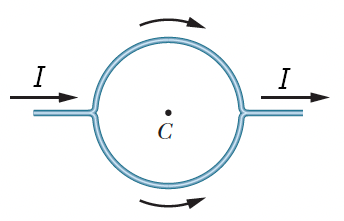
\includegraphics[width=0.50\textwidth]{./images/problems/lect05_wire_splitting_semicircular_arcs_2}\\
   \end{center}
   What is the magnetic field at the centre $C$ of the resulting circular loop?
   Justify your answer.
 \end{blockexmplque}

\end{frame}

%
%
%

\begin{frame}{Worked example: Magnetic field of two semi-circular arcs}

 The magnetic field $\vec{B}$ of a steady current $I$ at a given point $C$
 is given by the Biot-Savart law:
 \begin{equation*}
   \vec{B} = \frac{\mu_0I}{4\pi} \int_{wire} \frac{d\vec{\ell} \times \vec{r}}{r^3}
 \end{equation*}
 where, in the given problem at hand,
 $\vec{r}$ is the distance between the wire element $d\vec{\ell}$ and
 the point $C$.\\
 \vspace{0.3cm}

 In the given problem, the contribution of both straight conductor segments
 to the magnetic field at $C$ is zero.\\
 \vspace{0.3cm}

 This can be easily deduced from Biot-Savart law since,
 for the straight conductor segments, $d\vec{\ell}$ and $\vec{r}$
 are either parallel or antiparallel and, therefore,
 $d\vec{\ell} \times \vec{r}$ = 0.\\

\end{frame}

%
%
%

\begin{frame}{Worked example: Magnetic field of two semi-circular arcs}

 Each semi-circular segment gives a non-zero contribution to the
 magnetic field at $C$.\\
 \vspace{0.3cm}

 However, the symmetry of the problem suggests that
 the contributions from the two semi-circular segments have opposite
 directions and cancel out exactly.\\
 \vspace{0.3cm}

 Again, this can be easily deduced from Biot-Savart law:
 For any two diametrically opposite points of the circle formed by the
 two semi-circular segments, $d\vec{\ell}$ has the same but $\vec{r}$
 has the opposite direction. Therefore the $d\vec{\ell} \times \vec{r}$
 products for the two diametrically opposite points differ by a sign.\\
 \vspace{0.3cm}

 Therefore the total magnetic field at $C$ is zero.

\end{frame}

} % Worked example

% ------------------------------------------------------------------------------
% ------------------------------------------------------------------------------


%
% Worked example :
%

{
\problemslide

\begin{frame}{Worked example: Magnetic field of two wires on cylinder}

  \begin{blockexmplque}{Question}
    The figure below shows, in cross section, two long straight wires
    held against a plastic cylinder of radius $R$.
    Wire 1 carries current $I_1$ out of the page and is fixed in place at the
    left side of the cylinder. Wire 2 carries current $I_2$ out of the page
    and can be moved around the cylinder.
    \begin{columns}
      \begin{column}{0.45\textwidth}
        \begin{center}
          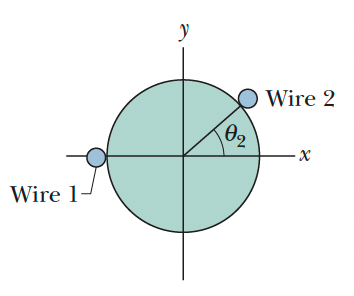
\includegraphics[width=0.95\textwidth]{./images/problems/lect05_wires_around_cylinder_1}\\
        \end{center}
      \end{column}
      \begin{column}{0.55\textwidth}
        When wire 2 is positioned at angle $\theta_2$, the magnetic field at the
        origin due to the two currents has magnitude $B$.
        Derive an expression for $\theta_2$, as a function of $B$, $I_1$ and$ I_2$.
      \end{column}
    \end{columns}
  \end{blockexmplque}

\end{frame}

%
%
%

\begin{frame}{Worked example: Magnetic field of two wires on cylinder}

  The magnetic field $\vec{B}_{1}$ at the origin due
  to a current $I_1$ out of the page is given by:
  \begin{equation*}
    \vec{B}_{1} = \frac{\mu_0 I_1}{2\pi R} \hat{y}
  \end{equation*}

  The magnetic field $\vec{B}_{2}$ at the origin due
  to a current $I_2$ out of the page is given by:
  \begin{equation*}
    \vec{B}_{2} = \frac{\mu_0 I_2}{2\pi R} \Big\{ sin\theta \hat{x} - cos\theta \hat{y} \Big\}
  \end{equation*}

  The total field $\vec{B}$ is given by the superposition principle:
  \begin{equation*}
    \vec{B} = \vec{B}_{1} + \vec{B}_{2}
  \end{equation*}

  The $x$ and $y$ components of the total field are given by:
  \begin{equation*}
    B_{x} = \cancelto{0}{B_{1x}} + B_{2x} =  \frac{\mu_0}{2\pi R} I_2 sin\theta
  \end{equation*}
  \begin{equation*}
    B_{y} = B_{1y} + B_{2y} =  \frac{\mu_0}{2\pi R} \Big( I_1 - I_2 cos\theta \Big)
  \end{equation*}
\end{frame}

%
%
%

\begin{frame}{Worked example: Magnetic field of two wires on cylinder}

  The magnitude of $\vec{B}$ is:
  \begin{equation*}
    B = \sqrt{B_{x}^2 + B_{y}^2}
  \end{equation*}

  Therefore:

  \begin{equation*}
    B = \sqrt{
      \Big\{ \frac{\mu_0}{2\pi R} I_2 sin\theta \Big\}^2 +
      \Big\{ \frac{\mu_0}{2\pi R} \Big( I_1 - I_2 cos\theta \Big) \Big\}^2 } \Rightarrow
  \end{equation*}

  \begin{equation*}
    B = \frac{\mu_0}{2\pi R} \sqrt{I_1^2 + I_2^2 - 2 I_1 I_2 cos\theta} \Rightarrow
  \end{equation*}

  \begin{equation*}
    cos\theta = \frac{I_1^2 + I_2^2 - 4\pi^2 R^2 B^2/\mu_0^2}{2 I_1 I_2}
  \end{equation*}

\end{frame}

} % Worked example


% ------------------------------------------------------------------------------
% ------------------------------------------------------------------------------

%
% Worked example :
%

{
\problemslide

\begin{frame}{Worked example: Current density of atmospheric ions}

  \begin{blockexmplque}{Question}
    At a point in the Earth’s atmosphere, He$^{++}$ ions in
    a concentration of 2.8 $\times$ 10$^{12}$ /m$^3$ are
    moving north at a speed of 2.0 $\times$ 10$^6$ m/s.
    Also, a 7.0 $\times$ 10$^{11}$ /m$^3$ concentration of
    O$_{2}^{-}$ ions is moving south at a speed of 6.2 $\times$ 10$^6$ m/s.
    Determine the magnitude and direction of the
    current density $\vec{j}$ at this point.
  \end{blockexmplque}

  The total current density $\vec{j}$ has two contributions:
  $\vec{j}_{He}$ because of the $He^{++}$ ions, and
  $\vec{j}_{O}$ because of the $O_2^{-}$ ions.\\

  Both represent a conventional current in the same direction:
  The positive $He^{++}$ ions flow to the North, creating a current with a direction
  from South to North, whereas the negative $O_2^{-}$ ions from to the South,
  creating a current with a direction which is again from South to North.
  Therefore, the two compponents can be added:
  \begin{equation*}
    j = j_{He} + j_{O}
  \end{equation*}

\end{frame}

%
%
%

\begin{frame}{Worked example: Current density of atmospheric ions}

  Generally, the current density $j_i$ because of charge carriers $i$ is given by:
  \begin{equation*}
    j_i = n_i q_i u_i
  \end{equation*}
  where $n_i$ is the numerical density of the charge carriers,
  $q_i$ is their charge, and $u_i$ is their drift velocity.
  Therefore, the total density can be written as:
  \begin{equation*}
    j = n_{He} q_{He} u_{He} + n_{He} q_{He} u_{He} \Rightarrow
  \end{equation*}
  \vspace{0.1cm}
  \begin{equation*}
    j = (2.8 \times 10^{12} \; /m^3) (2 x 1.6 x 10^{-19} \; C) (2.0 \times 10^{6} \; m/s) +
        %(7.0 \times 10^{11} \; /m^3) (1.6 x 10^{-19} \; C) (6.2 \times 10^{6} \; m/s)\Rightarrow
  \end{equation*}
  \begin{equation*}
  %j = (2.8 \times 10^{12} \; /m^3) (2 x 1.6 x 10^{-19} \; C) (2.0 \times 10^{6} \; m/s) +
        (7.0 \times 10^{11} \; /m^3) (1.6 x 10^{-19} \; C) (6.2 \times 10^{6} \; m/s)\Rightarrow
  \end{equation*}
  \vspace{0.1cm}
  \begin{equation*}
    j = 2.5 \; A/m^2
  \end{equation*}

\end{frame}

} % Worked example


% ------------------------------------------------------------------------------
% ------------------------------------------------------------------------------

%
% Worked example :
%

{
\problemslide

\begin{frame}{Worked example: Measuring Earth's magnetic field}

  \begin{blockexmplque}{Question}
    An experiment on the Earth’s magnetic field is being carried out 1.00 m
    from an electric cable. What is the maximum allowable current in the
    cable if the experiment is to be accurate to $\pm$2\%?
  \end{blockexmplque}

  The total magnetic field measured by the device is:
  \begin{equation*}
    \vec{B} = \vec{B}_{Earth} + \vec{B}_{wire}
  \end{equation*}
  where $\vec{B}_{Earth}$ is the magnetic field of the Earth, and
  $\vec{B}_{wire}$ is the magnetic field of the wire.\\
  \vspace{0.2cm}

  If we want the measurement of $B$ to represent $B_{Earth}$ to within 2\%,
  there is an upper limit on the strength of $B_{wire}$:
  \begin{equation*}
    B_{wire} \le 0.02 B_{Earth}
  \end{equation*}

\end{frame}

%
%
%

\begin{frame}{Worked example: Measuring Earth's magnetic field}

  The magnetic field of the wire, as a function of the distance $r$
  from the wire and the current $I$ in the wire, is given by:
  \begin{equation*}
    B_{wire} = \frac{\mu_0 I}{2\pi r}
  \end{equation*}

  Using this expression for $B_{wire}$, the previous upper limit yields:
  \begin{equation*}
    \frac{\mu_0 I}{2\pi r} \le 0.02 B_{Earth} \Rightarrow
    I \le 0.02 \frac{2\pi r B_{Earth}}{\mu_0}
  \end{equation*}

  Therefore, the maximum alloweable current has a value of $I_{max}$
  given by:
  \begin{equation*}
    I_{max} = 0.02 \frac{2\pi r B_{Earth}}{\mu_0} \Rightarrow
  \end{equation*}

  \begin{equation*}
    I_{max} = 0.02 \frac{2\pi (1\; m) (0.5\times 10^{-5}\; T)}
                        {4\pi \times 10^{-7} \; T\cdot m/A}
            = 5 \; A
  \end{equation*}

\end{frame}

} % Worked example
% ------------------------------------------------------------------------------
% ------------------------------------------------------------------------------

%
% Programming
%

{
\programmingslide

%
%
%

\begin{frame}{PHYS201 scientific programming task for Lecture \thislecture}

  Background information: {\bf Making a (conventional) neutrino beam}\\

  \begin{columns}
    \begin{column}{0.78\textwidth}
      \centering
      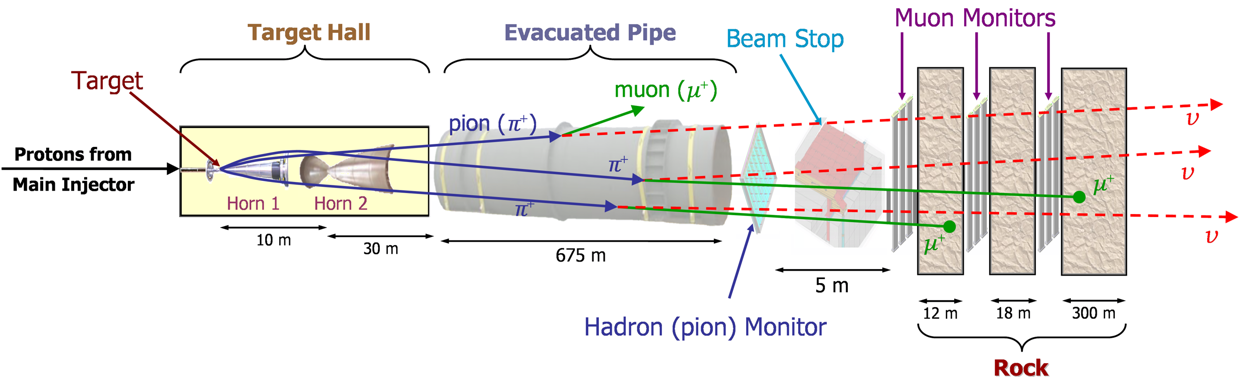
\includegraphics[width=0.95\textwidth]{./images/schematics/numi.png}\\
      \vspace{0.2cm}
      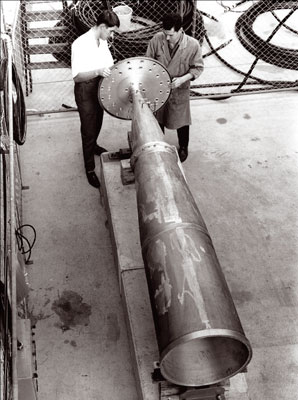
\includegraphics[width=0.32\textwidth]{./images/photos/beam_horn_old_1.jpg}
      \hfill
      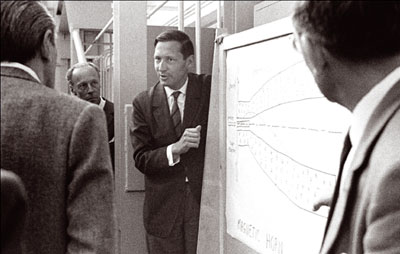
\includegraphics[width=0.66\textwidth]{./images/photos/beam_horn_old_3.jpg}
    \end{column}
    \begin{column}{0.22\textwidth}
     \begin{block}{}
     {\scriptsize
      Where do our $\nu$'s come from?\\
      \vspace{0.3cm}
      $\pi^{+} \rightarrow {\color{red}\nu_{\mu}} + \mu^{+}$\\
      $\pi^{-} \rightarrow {\color{magenta}\bar{\nu}_{\mu}} + \mu^{-}$\\
      $\mu^{+} \rightarrow {\color{magenta}\bar{\nu}_{\mu}} + {\color{blue}\nu_{e}} + e^{+}$\\
      $\mu^{-} \rightarrow {\color{green}\bar{\nu}_{e}} + {\color{red}\nu_{\mu}} + e^{-}$\\
      $K^{+} \rightarrow {\color{red}\nu_{\mu}} + \mu^{+}$\\
      $K^{+} \rightarrow {\color{blue}\nu_{e}} + \pi^{0} + e^{+}$\\
      $K^{+} \rightarrow {\color{red}\nu_{\mu}} + \pi^{0} + \mu^{+}$\\
      $K^{-} \rightarrow {\color{magenta}\bar{\nu}_{\mu}} + \mu^{-}$\\
      $K^{-} \rightarrow {\color{green}\bar{\nu}_{e}} + \pi^{0} + e^{-}$\\
      $K^{-} \rightarrow {\color{magenta}\bar{\nu}_{\mu}} + \pi^{0} + \mu^{-}$\\
      $K_{L}^{0} \rightarrow {\color{magenta}\bar{\nu}_{\mu}} + \pi^{+} + \mu^{-}$\\
      $K_{L}^{0} \rightarrow {\color{red}\nu_{\mu}} + \pi^{-} + \mu^{+}$\\
      $K_{L}^{0} \rightarrow {\color{green}\bar{\nu}_{e}} + \pi^{+} + e^{-}$\\
      $K_{L}^{0} \rightarrow {\color{blue}\nu_{e}} + \pi^{-} + e^{+}$\\
    }
    \end{block}
    \end{column}
  \end{columns}

\end{frame}


%
%
%

\begin{frame}{PHYS201 scientific programming task for Lecture \thislecture}

  Background information: {\bf The hadron hose}\\
  \vspace{0.3cm}
  {\small
  This is an additional {\bf focusing element}.
  It is a wire located in the decay pipe, downstream of the target and
  focussing horns. The wire is pulsed with current creating a toroidal
  magnetic field within the decay volume.\\
  See {\tt \color{blue} J.Hylen et al., https://arxiv.org/pdf/hep-ex/0210051.pdf}\\
  }
  \vspace{0.3cm}
  \begin{center}
    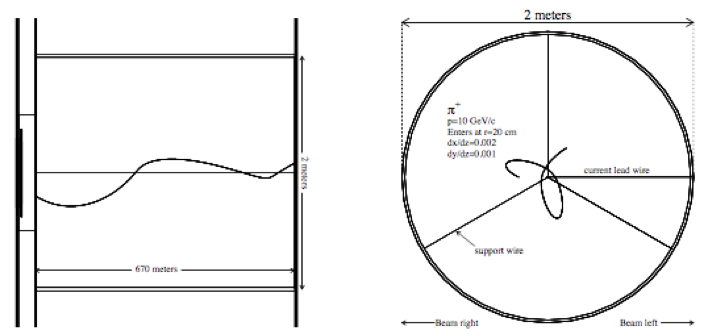
\includegraphics[width=0.75\textwidth]{./images/schematics/hadron_hose_trajectories.png}\\
    {\scriptsize Sample orbit for a 10 GeV $\pi^{+}$.}
  \end{center}
\end{frame}


%
%
%

\begin{frame}{PHYS201 scientific programming task for Lecture \thislecture}

\begin{itemize}
  \item Write a program to {\bf visualise trajectories of charged particles}
        moving in the magnetic field produced by the hadron hose.
  \vspace{0.3cm}
  \item In this lecture, we studied the two main elements for this calculation.
        \begin{itemize}
          \item The magnetic field produced by a long wire.
          \item The magnetic force on a moving electric charge.
        \end{itemize}
  \item The Runge-Kutta method (look it up) can be used for solving the equation
        of motion numerically and calculating the trajectories.
  \vspace{0.3cm}
  \item Assume that the decay pipe has a diameter of 2 m and a length of 700 m.
        Positively-charged pions, with a lifetime of 2.6 $\times$ 10$^{-8}$ $\mu$s
        enter the decay pipe from the centre of its upstream face.\\
        The pions have energies which are uniformly distributed in the 1-5 GeV range,
        and their direction is isotropic in the $\theta$ = $\pm$10$^{o}$ range,
        where $\theta$ is the angle between the hose and the pion direction.\\
        {\bf Optimize the hose current}, so as to maximize the number of pion decays
        within the decay volume and, hence, the neutrino flux.
\end{itemize}

\end{frame}


} % programming


% ------------------------------------------------------------------------------
% ------------------------------------------------------------------------------
